\documentclass[12pt, titlepage]{article}

\usepackage{float}
\usepackage{geometry}
\usepackage{booktabs}
\usepackage{tabularx}
\usepackage{hyperref}
\usepackage{siunitx}
\hypersetup{
    colorlinks,
    citecolor=blue,
    filecolor=black,
    linkcolor=red,
    urlcolor=blue
}
\usepackage[round]{natbib}
\usepackage{amsmath, mathtools}

\input{../Comments}
%% Common Parts

\newcommand{\progname}{Baja Dynamics} % PUT YOUR PROGRAM NAME HERE
\newcommand{\authname}{Team \#17, Team Name
\\ Grace McKenna
\\ Travis Wing
\\ Cameron Dunn
\\ Kai Arseneau} % AUTHOR NAMES                  

\usepackage{hyperref}
    \hypersetup{colorlinks=true, linkcolor=blue, citecolor=blue, filecolor=blue,
                urlcolor=blue, unicode=false}
    \urlstyle{same}
                                


\newcommand{\refdata}[2]{
  \href{https://github.com/gr812b/CVT-Simulator/blob/main/experimental-data/#1
  }{\texttt{#2}}}


\begin{document}

\title{System Verification and Validation Plan for \progname{}} 
\author{\authname}
\date{\today}
	
\maketitle

\pagenumbering{roman}

\section*{Revision History}

\begin{tabularx}{\textwidth}{p{3cm}p{2cm}X}
\toprule {\bf Date} & {\bf Version} & {\bf Notes}\\
\midrule
October 11th, 2024 & 0 & First version of VnV plan\\
\bottomrule
\end{tabularx}

~\\

\newpage

\tableofcontents

\listoftables
\wss{Remove this section if it isn't needed}

\listoffigures
\wss{Remove this section if it isn't needed}

\newpage

\section{Symbols, Abbreviations, and Acronyms}

\begin{table}[h]
  \raggedright
  \begin{tabular}{l l} 
    \toprule		
    \textbf{acronym} & \textbf{definition}\\
    \midrule
    CD & Continuous Development\\
    CI & Continuous Integration\\ 
    CVT & Continuous Variable Transmission\\
    FR & Functional Requirement\\
    GPS & Global Positioning System\\
    IMU & Inertial Measurement Unit\\
    GUI & Graphical User Interface\\
    IM & Instance Model\\
    MG & Module Guide\\
    MIS & Module Interface Specification\\
    MSE & Mean Squared Error\\
    NFR & Nonfunctional Requirement\\
    PR & Pull Request\\
    RPM & Revolutions Per Minute\\
    SRS & Software Requirements Specification\\
    VnV & Verification and Validation\\
    \bottomrule
  \end{tabular}
  \caption{Verification and Validation Acronyms}
  \label{tab:vnv_acronyms}
\end{table}

\newpage

\pagenumbering{arabic}

\noindent This document serves as a guide for how we plan to verify and validate the \progname{} system.
Within is a detailed plan of all the tests that will be conducted to ensure that the system is functioning as intended.
The document is divided into several sections going from the general plan to the specific tests that will be conducted.
On the verification side, the document lists all all the tests that will be conducted to verify the performance of the system.
The tests are divided into functional and nonfunctional requirements and then separate system and unit test for each.
There are also multiple checklist in place to verify that all the requirements both within and outside the document are met.
On the validation side, the document outlines all the plans in place to validate the results of the system.
This includes how we plan to compare our results against real world data and how we plan to validate the usability of the system.
Overall, this document comprehensively outlines all the plans in place to verify the system and validate its results.

\section{General Information}

This section serves as an overall summary of the verification and validation plan.
It includes a summary of the project and the overall objectives of the VnV plan.
The relevant documentation and other specifications are also listed.
In summary, this section provides a high level overview of the VnV plan.

\subsection{Summary}

The software that will be tested is the \progname{}, this is a system that simulates the Continuously Variable Transmission (CVT) system of a Baja vehicle.
The system has three components, a user interface which will allow the user to input the parameters of the CVT system and visualize the output of the simulation.
A mathematical component that will take the input parameters and simulate the CVT system.
There is also a 3D model component that will display the some models of the CVT system. 
Each of these components covered will be verified and validated to ensure that the system is functioning as intended.

\subsection{Objectives}

\noindent The objectives of testing our CVT system are to ensure the accuracy and reliability of our outputs. 
This includes evaluating that our mathematical model provides correct outputs based on provided input parameters specifically looking at the calculations of RPM, velocity, acceleration, distance, torque of the engine, clamping forces, CVT ratio, Torque and Belt slippage. 
We aim to emphasize the description over specification to make the CVT's system's behavior understandable by demonstrating how input changes influence the outputs.
We will verify that our 3D model and user interface allow users to easily input parameters to the system and interpret meaningful results. 
Our validation tests will focus on graphical models based on current available data to describe how the outputs should behave. 
We will aim to quantify these results by analyzing the difference between expected versus actual output. 
By referencing our outputs to real world data we can validate the accuracy of our mathematical model.
We will conduct useability testing to ensure that the interface is intuitive and allows users to easily input parameters, visualize results and understand the performance of the CVT.
\\
\noindent For our project attempting to optimize our systems outputs will be considered out of scope. 
Additionally, we will not verify any third party libraries used in our software as we assume that this has been previously validated. 

\subsection{Challenge Level and Extras}

The challenge level of this project is general.\\
\newline
The extras for this project are the following:\\
\textbf{Validation Report}
{\begin{itemize}
  \item The system will undergo validation testing to verify that accuracy of the simulation.
  \item The validation report will be included in the final documentation.
\end{itemize}}
{\noindent}
\textbf{Usability Testing}
{\begin{itemize}
  \item The system will undergo usability testing by members of the McMaster Baja team to ensure that
  the user interface is intuitive and easy to use.
  \item We will compile the results of the usability testing into a report that will be included in the final documentation.
\end{itemize}}

\subsection{Relevant Documentation}

\noindent \textbf{Software Requirements Specification} \citet{SRS}
\newline
This document is relevant because it it list all the requirements that the system should have and specifies how they should be achieved.
Requirements serve an important role in the verification process as the metric for determining if the system is functioning as intended.
When we do the verification of the system we will compare the system's capabilities and outputs to the requirements from the SRS document.
This will tell us what parts of the system are working as intended and which need to be changed or updated.
For validation, the specification serves and equivalent role as the metric for determining if the system is implemented correctly.
The specifications will be compared with the implementations of the system to see if they correspond.
If they do not, then the system will need to be updated so the the implementations match with the specifications.
Overall, the SRS document is important for verification and validation as it provides the metrics for determining their success.
\bigskip
\newline
\textbf{Module Guide}
\newline
The Module Guide will serve as a reference for the components of the system.
Each module listed in the MG will have a corresponding test case in the VnV plan.
\bigskip
\newline
\textbf{Module Interface Specification}
\newline
The Module Interface Specification serves as a reference for the functions and methods of the system.
Each function and method listed in the MIS will have a corresponding test case in the VnV plan.
\bigskip
\newline
\textbf{Verification and Validation Report}
\newline
The Verification and Validation Report will be referenced to ensure that all the components of the system have been verified and validated.

\section{Plan}

This section outlines the overall plans for the verification and validation of the system.
This includes our approaches, techniques and tools that will be used.
Our approaches our outlined and each person's role is specified.
There is also a plan listed for both the verification and validation along with an implementation specification.
Any tools that we plan to use to automate the process are also listed in this section.
Overall this section details how we plan to verify and validate the system.

\subsection{Verification and Validation Team}

\newgeometry{left=0.5cm, right=0.5cm, top=2cm, bottom=2cm}
\begin{table}[h!]
  \centering
  \begin{tabular}{|p{3cm}|p{3cm}|p{10cm}|}
  \hline
  \textbf{Name} & \textbf{Role} & \textbf{Responsibilities} \\
  \hline
  Kai Arseneau & Data Verification Lead & Analyzes data outputs to ensure trends align with expected performance and validates consistency across simulation runs. \\
  \hline
  Travis Wing & GUI Verification Lead & Ensures user interface functionality and usability, verifying that GUI elements accurately reflect simulation data and respond as intended. \\
  \hline
  Cameron Dunn & Experimental Data Comparison Lead & Compares simulation outputs to real-world data and scripts, verifying the simulation's accuracy and adjusting model parameters as needed. \\
  \hline
  Grace McKenna & Quality Assurance Lead & Conducts comprehensive testing of simulation processes and components, identifying and documenting issues, and ensuring overall software reliability. \\
  \hline
  Ariel Wolle & Team Lead & Supports the project by overseeing resources and approving initiatives that facilitate enhanced data acquisition or other verification efforts. \\
  \hline
  Daksh Mathur &  Data Acquisition Lead & Acts as the primary contact for real-world data acquisition, providing essential data for validation and supporting data needs beyond the project group. \\
  \hline
  Benjamin Waldie & Mechanical Advisor & Collaborates with the team to validate mathematical models within the simulation, ensuring mechanical accuracy and guiding technical correctness. \\
  \hline
  Duncan Shearer and Leonardo Ansari & Primary User & Utilizes the simulation tool to tune CVTs, providing feedback on tool usability and functionality to ensure it meets real-world tuning needs. \\
  \hline
  Dr. Spencer Smith & Project Advisor / Supervisor & Reviews and provides final feedback, ensuring verification meets project standards and advising on methodology improvements. \\
  \hline
  \end{tabular}
  \caption{Verification and Validation Team for CVT Simulation Project}
  \label{tab:vnv_team}
\end{table}
\restoregeometry
    
\subsection{Data Collection}

\noindent To ensure accurate validation of our CVT simulation outputs, the McMaster Baja Racing team employs a robust data collection system. This system, overseen by the Data Acquisition Lead, records GPS data (including position and velocity), Inertial Measurement Unit (IMU) data, engine speed, and wheel speed during structured testing sessions. These testing days are designed to maintain predictable and repeatable conditions, providing high-quality, reliable data.

The collected data will be distributed among the CVT team members, ensuring alignment between simulation predictions and physical testing outcomes. References to specific data metrics appear throughout this document, providing context for how each aspect of collected data supports the validation objectives outlined.
\subsection{SRS Verification Plan}

\noindent To ensure that the SRS document is accurate and complete, we will be conducting a series of reviews.
These reviews will be conducted by the team, our supervisor, and our stakeholders.
The team will use the below checklist to verify the quality of the SRS document:
\begin{itemize}
  \item Review the SRS document for spelling, grammatical and formatting errors
  \item Check the applicability of each theoretical models
  \item Check the usefulness of each data definitions
  \item Check the validity of each instance models
\end{itemize}

\subsubsection*{Review Meetings}
We will conduct meetings with experienced team members and alumni to review the SRS document.
These meetings will focus on the theoretical models, data definitions, and instance models.
We will also conduct a practicality check to ensure that all requirements are feasible and measurable.
Finally the assumptions will also be verified to ensure that they won't negatively impact the accuracy of the simulation.

\subsubsection*{Baja Team Review}
Talk here about sharing the document to the team as a whole, include a checklist and receive issues on github.

We will share the SRS document with the entire McMaster Baja Racing team for review.
This will allow us to get feedback from a wide range of people with different backgrounds and experiences.
The team will use the checklist provided above as a guide for their reviews.
Afterwards we will compile all of their feedback and address any issues that they have raised.

\subsubsection*{Capstone Team Testing}

We will conduct unit tests on the mathematical models provided by the SRS document.
These will be done on their implementations to ensure that they are functioning as intended.
If any issues are found, we will reference the assumptions and requirements in the SRS document to determine the cause of the issue.
Additionally, the traceability matrix will be used to ensure that the mapping between requirements and goals is logical. 

\subsection{Design Verification Plan}

\noindent To ensure that the CVT system is functional and accurate, a design verification plan will be conducted on the system. 
The components of the system that will be tested are the graphical user interface, data output and visualization and the mathematical model. 
The design verification plan will include, reviews from fellow classmates, stakeholder reviews and specification testing based on the functional and nonfunctional requirements of the system. 
The system will receive Stakeholder review providing us with relevant feedback on the functionality and interface of our design.
The system will undergo reviews from fellow classmates, providing our team with quality feedback from an outside perspective. 
A checklist has been designed below to which fellow classmates and stakeholders can use to verify the system.  


\begin{enumerate}
  \item For each functional requirement there is a at least one corresponding system test.
  \item For each non functional requirement there is a at least one corresponding system test.  
  \item The system tests contain tests for boundary cases for user inputs, empty inputs and edge cases. 
  \item Each instance model (IM) within the SRS document shall correspond to a unit test. 
  \item Each function written in our mathematical python model shall correspond to at least one unit test. 
  \item There exists system tests for each component: user interface, mathematical model, data visualization and 3D model. 
\end{enumerate}
\subsection{Verification and Validation Plan Verification Plan}

To ensure that the Verification and Validation Plan is sufficient, this document will undergo a verification plan.
This plan will review the contents of the document to make sure that all necessary components are included.
It will be reviewed by our team, supervisor, stakeholders and classmates.
Below is a checklist to use as reference for the verification of the Verification and Validation Plan.
\bigskip
\newline
\textbf{Overall}
\begin{itemize}
  \item The document is well organized and easy to follow
  \item The document is free of spelling, grammatical and formatting errors
  \item The document is consistent with all other documentation and implementation
  \item The document is complete and has all components filled out
  \item References are included and correct
\end{itemize}
\noindent
\textbf{Section 1}
\begin{itemize}
  \item Tables included are relevant and necessary
  \item Tables include are correct and formatted properly
  \item Introduction sufficiently introduces the document
\end{itemize}
\noindent
\textbf{Section 2}
\begin{itemize}
  \item Roadmap effective summarizes the section
  \item Summary effectively summarizes the document
  \item Objectives are clear and concise
  \item Challenge Level correct and Extras are appropriate
  \item Relevant Documentation is matching and descriptive
\end{itemize}
\noindent
\textbf{Section 3}
\begin{itemize}
  \item Roadmap effective summarizes the section
  \item Team roles allocated properly and effectively
  \item SRS Verification Plan includes all necessary components in the checklist
  \item Design Verification Plan includes all necessary components in the checklist
  \item VnV Plan Verification Plan includes all necessary components in the checklist
  \item Implementation Verification Plan includes all techniques that are used
  \item Automated Testing and Verification Tools includes all tools that are used
  \item Software Validation Plan includes all external data that is used
\end{itemize}
\noindent
\textbf{Section 4}
\begin{itemize}
  \item Roadmap effective summarizes the section
  \item All functional requirements have corresponding system tests
  \item All nonfunctional requirements have corresponding system tests
  \item Traceability table between test cases and requirements is clear
\end{itemize}
\noindent
\textbf{Section 5}
\begin{itemize}
  \item Roadmap effective summarizes the section
  \item Unit Testing Scope is correctly defined
  \item All functional requirements have corresponding unit tests
  \item All nonfunctional requirements have corresponding unit tests
  \item Unit tests are properly grouped into their respective modules
  \item Traceability table between test cases and modules is clear and includes all modules
\end{itemize}
\noindent
\textbf{Section 6}
\begin{itemize}
  \item Roadmap effective summarizes the section and includes all additions
  \item Additional information is relevant and necessary
  \item Included sections are informative and properly filled out
\end{itemize}


\subsection{Implementation Verification Plan}

For the implementation verification plan, we will be using many techniques to ensure that the system is functioning as intended.
We will use the unit tests listed in the this document as well as other common testing techniques.
It will be required that all unit tests are run and pass for any PRs to be merged into their parent branch.
We will be doing code inspections during development by ensuring that all code is reviewed by at least one other team member before merging.
Static analyzers will also be used throughout development to ensure a high quality codebase and will be integrated into our CI/CD pipeline.
Before major milestones, full code walkthroughs will be conducted which is enforced by all team members needing to approve merges into main.

\subsection{Automated Testing and Verification Tools}

  \noindent We will be using a wide variety of tools for automated testing and verification.
  We will use separate tools for our Unity C\# frontend and python backend.
  \bigskip
  \newline
  For the python backend we will be using the following tools:
  \begin{itemize}
    \item [\textbf{flake8}] - A Python linter that checks for PEP8 compliance.
    \item [\textbf{black}] - A Python code formatter that will ensure consistent code style.
    \item [\textbf{unittest}] - Python's built-in testing framework that will be used for unit testing.
    \item [\textbf{coverage}] - A testing framework for Python that will be used for code coverage.
  \end{itemize}

  \bigskip
  \noindent For the Unity C\# frontend we will be using the following tools:
  \begin{itemize}
    \item [\textbf{SonarLint}] - C\# linter that checks for code quality and security vulnerabilities.
    \item [\textbf{StyleCop}] - C\# linter that checks for code style and formatting.
    \item [\textbf{UTF}] - A testing framework for C\# that will be used for unit testing.
    \item [\textbf{UTR}] - A testing framework for Unity that will be used for unit testing and code coverage.
  \end{itemize}

  \noindent Additionally, we will be using GitHub Actions to automate our testing process.
  This will be done to ensure CI/CD and that our tests are run automatically on every push to the repository.
\subsection{Software Validation Plan}

\noindent We plan on using data collected from the McMaster Baja team to validate the accuracy of our simulation.
Some of the values we are able to collect include:
\begin{itemize}
  \item Primary RPM
  \item Secondary RPM
  \item CVT Ratio (from Primary and Secondary RPM)
  \item Wheel Speed
  \item GPS Speed
  \item GPS Position
  \item Acceleration
\end{itemize}

\noindent To validate this data against our simulation we plan on creating a script to compare them.
This script will compute the MSE between the two datasets and also plot that error over time.
Plotting the error will allow us to see in what scenarios the simulation is least accurate.
This will allow us to better diagnose the issues and allocate our resources to fix them.

\section{System Tests}

Found below are all of the system tests that will be conducted to verify the system.
These tests are split based on if they are for functional or nonfunctional requirements.

\subsection{Tests for Functional Requirements}

This section outlines all the system tests that will be conducted to verify the requirements of the system.
Each set of tests relate to one requirement from the SRS document.

\subsubsection*{Standard Simulation Inputs}
\label{sec:standard_inputs}
The standard simulation inputs for the CVT system are as follows.
\begin{enumerate}
  \item Primary Pulley System:
  \begin{itemize}
    \item Flyweight
    \item Ramp Geometry
    \item Spring rate
    \item Spring pretension
  \end{itemize}
  \item Secondary Pulley System:
  \begin{itemize}
    \item Helix Geometry
    \item Torsional spring rate
    \item Compressional spring rate
    \item Spring pretension
  \end{itemize}
  \item Vehicle Characteristics:
  \begin{itemize}
    \item Car weight
    \item Driver weight
    \item Traction
    \item Angle of incline
  \end{itemize}
\end{enumerate}

\subsubsection*{Standard Simulation State}
\label{sec:standard_state}
The standard simulation state for the CVT system is as follows.
\begin{itemize}
  \item Vehicle is stationary.
  \item The engine's angular velocity is at $\omega_\text{idle}$.
  \item The CVT system is in a neutral state, unshifted.
  \item The belt is stationary.
\end{itemize}

\subsection{Tests for Functional Requirements}

\wss{Subsets of the tests may be in related, so this section is divided into
  different areas.  If there are no identifiable subsets for the tests, this
  level of document structure can be removed.}

\wss{Include a blurb here to explain why the subsections below
  cover the requirements.  References to the SRS would be good here.}

\subsubsection{Area of Testing1}

\wss{It would be nice to have a blurb here to explain why the subsections below
  cover the requirements.  References to the SRS would be good here.  If a section
  covers tests for input constraints, you should reference the data constraints
  table in the SRS.}
		
\paragraph{Velocity}

\begin{enumerate}

\item{Velocity test-1\\}

Control: Manual
					
Initial State: The state values from Section~\ref{sec:standard_state}.

Input: The input values from Section~\ref{sec:standard_inputs}.
					
Output: The resulting graph should show a velocity that is a monotonically increasing function over time, starting from zero and remaining below $v_\text{max}$, which reflects the vehicle’s physical limits. A typical output graph will look similar to the one shown in Figure~\ref{fig:velocity_graph}.

Test Case Derivation: \wss{Justify the expected value given in the Output field}
					
How test will be performed: 
					
\item{test-id2\\}

Control: Manual versus Automatic
					
Initial State: 
					
Input: 
					
Output: \wss{The expected result for the given inputs}

Output: Mean squared error between the simulated velocity and the experimental velocity.

Test Case Derivation: Data from the simulation should closely match the experimental data collected from the physical car.

How test will be performed: The script will run with the provided inputs. After execution is complete, the output of the simulation will be compared to experimental data from the physical car to ensure that the simulation is accurate.

\end{enumerate}

\subsubsection{Area of Testing2}

...

\subsection{Tests for Nonfunctional Requirements}

\wss{The nonfunctional requirements for accuracy will likely just reference the
  appropriate functional tests from above.  The test cases should mention
  reporting the relative error for these tests.  Not all projects will
  necessarily have nonfunctional requirements related to accuracy.}

\wss{For some nonfunctional tests, you won't be setting a target threshold for
passing the test, but rather describing the experiment you will do to measure
the quality for different inputs.  For instance, you could measure speed versus
the problem size.  The output of the test isn't pass/fail, but rather a summary
table or graph.}

\wss{Tests related to usability could include conducting a usability test and
  survey.  The survey will be in the Appendix.}

\subsubsection{CVT Dynamics}

This section provides tests to verify the CVT dynamics of the system.
They are based on the following functional requirements from the SRS document.
Listed is each requirement and how the tests verify each one.
\begin{itemize}
  \item [R1:] Verifies the mathematical modeling of the CVT system
  \item [R5:] Verifies the calculations of the primary clamping force
  \item [R6:] Verifies the calculations of the secondary clamping force
  \item [R7:] Verifies the calculations of the sheave acceleration
  \item [R8:] Verifies the calculations of the belt acceleration
  \item [R9:] Verifies the calculations of RPM and engine torque
\end{itemize}

\paragraph{Clamping forces}

\begin{enumerate}
  
  \item{Clamping forces test-1\\}
  
  Control: Manual
            
  Initial State: The state values from Section~\ref{sec:standard_state}.
  
  Input: The input values from Section~\ref{sec:standard_inputs}.
            
  Output: The resulting graphs should show a clamping force against engine angular velocity beginning an initial minimum value, which should then rise to a peak before falling during the shifting phase. Suboptimal parameters may lead to a clamping force that is too low or too high, but a similar shape nonetheless. A typical output graph will look similar to the one shown in Figure~\ref{fig:clamping_force_graph}.
  
  Test Case Derivation: This behaviour is resulting from ideal tuning parameters, and may vary depending on inputs. Ramp and helix geometry will both have a major impact on the shape of these graphs, while weight and spring constants will affect the magnitude.
  
  How test will be performed: The script will run with the provided inputs. After execution is complete, the output will be visualized as a graph. Visual inspection will follow against Figure~\ref{fig:clamping_force_graph} for confirmation of expected behaviour.
  
\end{enumerate}

\subsubsection{Area of Testing2}

...

\subsection{Traceability Between Test Cases and Requirements}

\wss{Provide a table that shows which test cases are supporting which
  requirements.}

\section{Unit Test Description}

\wss{This section should not be filled in until after the MIS (detailed design
  document) has been completed.}

\wss{Reference your MIS (detailed design document) and explain your overall
philosophy for test case selection.}  

\wss{To save space and time, it may be an option to provide less detail in this section.  
For the unit tests you can potentially layout your testing strategy here.  That is, you 
can explain how tests will be selected for each module.  For instance, your test building 
approach could be test cases for each access program, including one test for normal behaviour 
and as many tests as needed for edge cases.  Rather than create the details of the input 
and output here, you could point to the unit testing code.  For this to work, you code 
needs to be well-documented, with meaningful names for all of the tests.}

\subsection{Unit Testing Scope}

\wss{What modules are outside of the scope.  If there are modules that are
  developed by someone else, then you would say here if you aren't planning on
  verifying them.  There may also be modules that are part of your software, but
  have a lower priority for verification than others.  If this is the case,
  explain your rationale for the ranking of module importance.}

\subsection{Tests for Functional Requirements}

\wss{Most of the verification will be through automated unit testing.  If
  appropriate specific modules can be verified by a non-testing based
  technique.  That can also be documented in this section.}

\subsubsection{Module 1}

\wss{Include a blurb here to explain why the subsections below cover the module.
  References to the MIS would be good.  You will want tests from a black box
  perspective and from a white box perspective.  Explain to the reader how the
  tests were selected.}

\begin{enumerate}

  \item{Engine test-1\\}
  
  Control: Manual
            
  Initial State: The state values from Section~\ref{sec:standard_state}.
  
  Input: The input values from Section~\ref{sec:standard_inputs}.
            
  Output: The resulting graph should show a decreasing relationship with forque and engine angular velocity, while having a peak in power at $\omega_\text{peak\_power}$. A typical output graph will look similar to the one shown in Figure~\ref{fig:engine_graph}.
  
  Test Case Derivation: These are given values as specs of the engine at full load. The engine should not significantly leave the bounds of these angular velocities.
  
  How test will be performed: The script will run with the provided inputs. After execution is complete, the output will be visualized as a graph. Visual inspection will follow against Figure~\ref{fig:engine_graph} for confirmation of expected behaviour.

\end{enumerate}

\subsubsection{User Interface}

This section provides tests to verify the User Interface of the system.
They are based on the following functional requirements from the SRS document.
Listed is each requirement and how the tests verify each one.
\begin{itemize}
  \item [R10:] Verifies the input parameters of the CVT can be adjusted
  \item [R11:] Verifies the other input parameters can be adjusted
  \item [R12:] Verifies the system provides a UI to change the input parameters
  \item [R13:] Verifies the system provides output in the form of graphs
  \item [R14:] Verifies the system lets users compare simulation data
  \item [R15:] Verifies the system lets users export simulation data
\end{itemize}

\begin{enumerate}
  \item{User Interface test-1\\}
  
  Control: Manual

  Initial State: Default input parameters are loaded
            
  Input: Change the input parameters with new values
            
  Output: Input parameters have been updated 
  
  Test Case Derivation: Based on FR10 and FR11, the user should be able to adjust each of the input parameters (within the limitations of the input itself).
  This includes CVT parameters such as weight, ramp geometry, spring rate and spring pretension as well as other parameters such as vehicle weight, driver weight, traction and angle of incline. 
  
  How test will be performed: Upon a fresh launch of the application, manually change each of the input parameters from the default values to a new value. 
             
  \item{User Interface test-2\\}
 
  Control: Automatic
            
  Initial State: Application has not been launched
            
  Input: Launch application
            
  Output: User interface for changing the input parameters is displayed
  
  Test Case Derivation: Based on FR12 validate that the system provides the user with a UI to change the input parameters.
  
  How test will be performed: Upon a fresh launch of the software, the system will assert whether the input parameter page is displayed or not. 
  \item {User Interface test-3\\}
  
  Control: Automatic
            
  Initial State: Simulation pre loaded with input parameters
            
  Input: Run simulation 
            
  Output: Graphical representation of simulation data is displayed to the user
  
  Test Case Derivation: Based on FR13, validate that the simulation produces output in the form of graphs.
  
  How test will be performed: The test will run the simulation with a set of pre made input parameters, then it will verify that whether or not a graph has been outputted. 
  \item {User Interface test-4\\}
  
  Control: Manual
            
  Initial State: Simulation has completed
            
  Input: Another simulation is run with different input parameters
            
  Output: Both simulations are displayed to the user for comparison
  
  Test Case Derivation: Based on FR14 validate that the system lets users compare simulation data.
  
  How test will be performed: After running two simulations with different input parameters, the user will be able to compare the two simulations to see the differences in the output.
  \item {User Interface test-5\\}
  
  Control: Manual
            
  Initial State: Simulation has completed
            
  Input: Select export data option
            
  Output: simulation data exported successfully
  
  Test Case Derivation: Based on the FR15 validate user can export simulation data after simulation has completed.
  
  How test will be performed: After simulation has completed successfully export the data and verify that it was exported in the correct format to the right location.

\end{enumerate}

  \subsubsection{Compatability}

  This section provides tests to verify the Compatability of the system.
They are based on the following functional requirements from the SRS document.
Listed is each requirement and how the tests verify each one.
\begin{itemize}
  \item [R16:] Verifies the application works on different types of computers
  \item [R17:] Verifies the application works on different operating systems
\end{itemize}

  \begin{enumerate}
  \item {Compatability test-1\\}
  
  Control: Manual
            
  Initial State: Application is not installed
            
  Input: Install application files
            
  Output: Applications installs and functions as expected
  
  Test Case Derivation: Based on FR16 and FR17, validate that the application can be installed and ran on different operating systems and types of computers. 
  
  How test will be performed: This test will be performed on two types of computers, a personal laptop and a desktop. On each of those types of computers it will be ran on each of the operating systems, Windows, Linux and MacOS to verify compatability with each OS and type of computer.

  \end{enumerate}

\subsection{Tests for Nonfunctional Requirements}

\noindent The nonfunctional requirements we will be testing for are accuracy, useability, maintainability, verifiability, understandability and reusability. 
Referencing the Nonfunctional requirements within the SRS document: NFR1: Accuracy, NFR4 Verifiability will reference the above tests given for the functional requirements. 
The Nonfunctional requirements related to useability and understandability (NFR2 and NFR 5 respectively) will reference the useability/understandability survey linked in the appendix.

\subsubsection{Accuracy}

The below test are to verify the accuracy of the system.
They are based on NFR1 from the SRS document.

\begin{enumerate}

\item{test-1\\}

Type: Manual
					
Initial State: The user has successfully installed the system on their device and completed the tests above for the functional requirements.
					
Input/Condition: The outputs of the functional tests: Position test-2, Velocity test-2, Acceleration test-2, Shift test-2 and Shift test-4. 
					
Output/Result: Based on the outputted MSE's from the functional requirement tests listed we will look at the various MSE's to estimate the accuracy. 
Each MSE is within 0.2 of 0.
					
How test will be performed: We will compare each MSE to the value of 0 as the closer the value to 0 the more accurate the prediction. An MSE with a range of 0-0.2 will indicate our system is accurate.

\end{enumerate}

\subsubsection{Useability}

The below test are to verify the useability of the system.
They are based on NFR2 from the SRS document.

\begin{enumerate}

\item{test-1\\}

Type: Manual
					
Initial State: 
					
Input/Condition: Users within the Primary User role as well as Baja team members are asked to rate how simple the navigation process of the main interface. 
They are asked to rate this on a scale of (1-5) 1 being extremely difficult and 5 being extremely easy with the other options being 4: somewhat easy, 3: neutral and 2: somewhat difficult. 
					
Output/Result: The average output rating from all users is greater than or equal to a 4(somewhat easy or above expectations).
					
How test will be performed: Each user in the test group will be provided with a survey which provides a series of questions and a scale for each option where 1 represents Poor, 2 represents below expectation, 3 represents satisfactory, 4 represents above average and 5 represents excellent.
The average rating will then be calculated and must be above or equal to 4 representing the system usability is above expectations.  

\item{test-2\\}
  
Type: Manual
            
Initial State: The user has successfully installed the system on their device.
            
Input/Condition: Users within the Primary User role as well as Baja team members are asked to rate the features inputting parameters, adjusting parameters, viewing data outputs and saving and exporting data on how easy it was to use each feature.
They are asked to rate this on a scale of (1-5) 1 being extremely difficult and 5 being extremely easy with the other options being 4: somewhat easy, 3: neutral and 2: somewhat difficult. 
            
Output/Result: The average output rating from all users for each listed feature is greater than or equal to a 4(somewhat easy or above expectations).
            
How test will be performed: Each user in the test group will be provided with a survey which provides a series of questions and a scale for each option where 1 represents Poor, 2 represents below expectation, 3 represents satisfactory, 4 represents above average and 5 represents excellent.
The average rating will then be calculated and must be above or equal to 4 representing the system usability is above expectations. 
  
\end{enumerate}

\subsubsection{Maintainability}

The below test are to verify the maintainability of the system.
They are based on NFR3 from the SRS document.

\begin{enumerate}

\item{test-1\\}

Type: Manual
					
Initial State: The completed system which includes, the finalized mathematical model, GUI and 3D model.  
					
Input/Condition: The 2023 McMaster Baja CVT's configuration. 
					
Output/Result: The amount of time taken and number of lines of code modified using the 2023 CVT.
					
How test will be performed: The test will be manually completed by the teams Quality Assurance Lead, where the amount of time and number of lines of code will be recorded when implementing the changes that correspond to the 2023 CVT configuration.

\end{enumerate}

\subsubsection{Verifiability}

The below test are to verify the verifiability of the system.
They are based on NFR4 from the SRS document.

\begin{enumerate}

\item{test-1\\}

Type: Manual
					
Initial State: The tests for the functional requirements and the Nonfunctional requirement test Accuracy test1 have been completed.
					
Input/Condition: The outputs of the functional tests: Position test1, Velocity test-1, Acceleration test-1, Shift test-, Shift test-1 and Shift test-3 will be run 30 times with the same input settings. 
					
Output/Result: The graphed behavior of each run is consistent each time.
					
How test will be performed: The outputs will be compared after each run to ensure that the behaviour of each run is consistent for the same tunning settings.

\end{enumerate}

\subsubsection{Understandability}

The below test are to verify the understandability of the system.
They are based on NFR5 from the SRS document.

\begin{enumerate}

\item{test-1\\}

Type: Manual.
					
Initial State: The user has successfully installed the system on their device.
					
Input/Condition: Users within the Primary User role as well as Baja team members are asked to rate how clear they found the features and functions within the system. 
They are asked to rate this on a scale of (1-5) 1 being extremely unclear and 5 being extremely clear with the other options being 4: somewhat clear, 3: neutral and 2: somewhat unclear. 
					
Output/Result: The average output rating from all users for each listed feature is greater than or equal to a 4(somewhat clear or above expectations).
					
How test will be performed: Each user in the test group will be provided with a survey which provides a series of questions and a scale for each option where 1 represents Poor, 2 represents below expectation, 3 represents satisfactory, 4 represents above average and 5 represents excellent.
The average rating will then be calculated and must be above or equal to 4, representing the systems understandability is above expectations.  

\item{test-2\\}

Type: Manual
					
Initial State: The user has successfully installed the system on their device.
					
Input/Condition: Users within the Primary User role as well as Baja team members are asked to rate their understanding of the simulation results and outputs. 
They are asked to rate this on a scale of (1-5) 1 being extremely unclear and 5 being extremely clear with the other options being 4: somewhat clear, 3: neutral and 2: somewhat unclear. 
					
Output/Result: The average output rating from all users for each listed feature is greater than or equal to a 4(somewhat clear or above expectations).
					
How test will be performed: Each user in the test group will be provided with a survey which provides a series of questions and a scale for each option where 1 represents Poor, 2 represents below expectation, 3 represents satisfactory, 4 represents above average and 5 represents excellent.
The average rating will then be calculated and must be above or equal to 4, representing the systems understandability is above expectations. 

\end{enumerate}

\subsubsection{Reusability}

The below test are to verify the reusability of the system.
They are based on NFR6 from the SRS document.

\begin{enumerate}

\item{test-1\\}
    
Type: Manual
              
Initial State: Completed system which includes, the finalized mathematical model, GUI and 3D model.  
              
Input/Condition: The 2023 McMaster Baja CVT's configuration. 
              
Output/Result: The amount of time taken and number of lines of code modified using the 2023 CVT.
              
How test will be performed: The test will be manually completed by the teams Quality Assurance Lead, where the amount of time and number of lines of code will be recorded when implementing the changes to correspond to the 2023 CVT.
This will indicate how long it will take for the system to be adapted to future CVT configurations. 
    
\end{enumerate}

\subsection{Traceability Between Test Cases and Requirements}


\begin{table}[H]
\centering
  \begin{tabular}{|c|c|}
    \hline
    \textbf{Requirement} & \textbf{Test(s)} \\ \hline
    R1 & Position test-2, Velocity test-2, Acceleration test-2, Shift test-4  \\ \hline
    R2 & Acceleration test-1 \\ \hline
    R3 & Velocity test-1 \\ \hline
    R4 & Position test-1 \\ \hline
    R5 & Clamping forces test-1 \\ \hline
    R6 & Clamping forces test-1 \\ \hline
    R7 & Shift test-1, Shift test-2, Shift test-3 \\ \hline
    R8 & Shift test-1, Shift test-2, Shift test-3 \\ \hline
    R9 & Engine test-1 \\ \hline
    R10 & User Interface test-1 \\ \hline
    R11 & User Interface test-1 \\ \hline
    R12 & User Interface test-2 \\ \hline
    R13 & User Interface test-3 \\ \hline
    R14 & User Interface test-4 \\ \hline
    R15 & User Interface test-5 \\ \hline
    R16 & Compatibility test-1 \\ \hline
    R17 & Compatibility test-1 \\ \hline
    \end{tabular}
    \caption{System Functional Requirements and Corresponding Tests}
    \label{tab:requirements_tests}
\end{table}

\begin{table}[h!]
  \centering
    \begin{tabular}{|c|c|}
      \hline
      \textbf{Requirement} & \textbf{Test(s)} \\ \hline
      NFR1 & Accuracy test-1  \\ \hline
      NFR2 & Useability test-1, Useability test-2 \\ \hline
      NFR3 & Maintainability test-1 \\ \hline
      NFR4 & Verifiability test-1 \\ \hline
      NFR5 & Understandability test-1, Understandability test-2 \\ \hline
      NFR6 & Reusability test-1 \\ \hline
      \end{tabular}
      \caption{System Nonfunctional Requirements and Corresponding Tests}
      \label{tab:requirements_tests}
  \end{table}

\section{Unit Test Description}

This section is not applicable to this version of this document, as the system is not yet implemented.
When implementation is completed, this section will be updated to include the unit tests that will be conducted.

\subsection{Unit Testing Scope}
N/A

\subsection{Tests for Functional Requirements}
N/A

\subsection{Tests for Nonfunctional Requirements}
N/A

\subsection{Traceability Between Test Cases and Modules}
N/A	

\bibliographystyle{plainnat}

\bibliography{../../refs/References}

\newpage

\section{Appendix}

\subsection{Symbolic Parameters}

The definition of the test cases will call for SYMBOLIC\_CONSTANTS.
Their values are defined in this section for easy maintenance.

\begin{table}[h]
  \raggedright
  \begin{tabular}{l l} 
    \toprule		
    \textbf{constant} & \textbf{value}\\
    \midrule
    $v_\text{max}$ & 16.67 m/s \\
    $\omega_{\text{idle}}$ & 180 rad/s \\
    $\omega_\text{max}$ & 420 rad/s \\
    $\omega_\text{peak\_power}$ & 6987.24 W \\
    \bottomrule
  \end{tabular}
  \caption{Verification and Validation Constants}
  \label{tab:vnv_constants}
\end{table}

\subsection{Usability Survey Questions?}

Useability/Understandability survey:
\url{https://forms.office.com/r/RkeDW31ZTS}

\subsection{Expected Graphs}
This section includes all referenced graphs for various tests. Please note that all values may not be accurate, and it is the shape that is being tested for.

\begin{figure}[H]
  \centering
  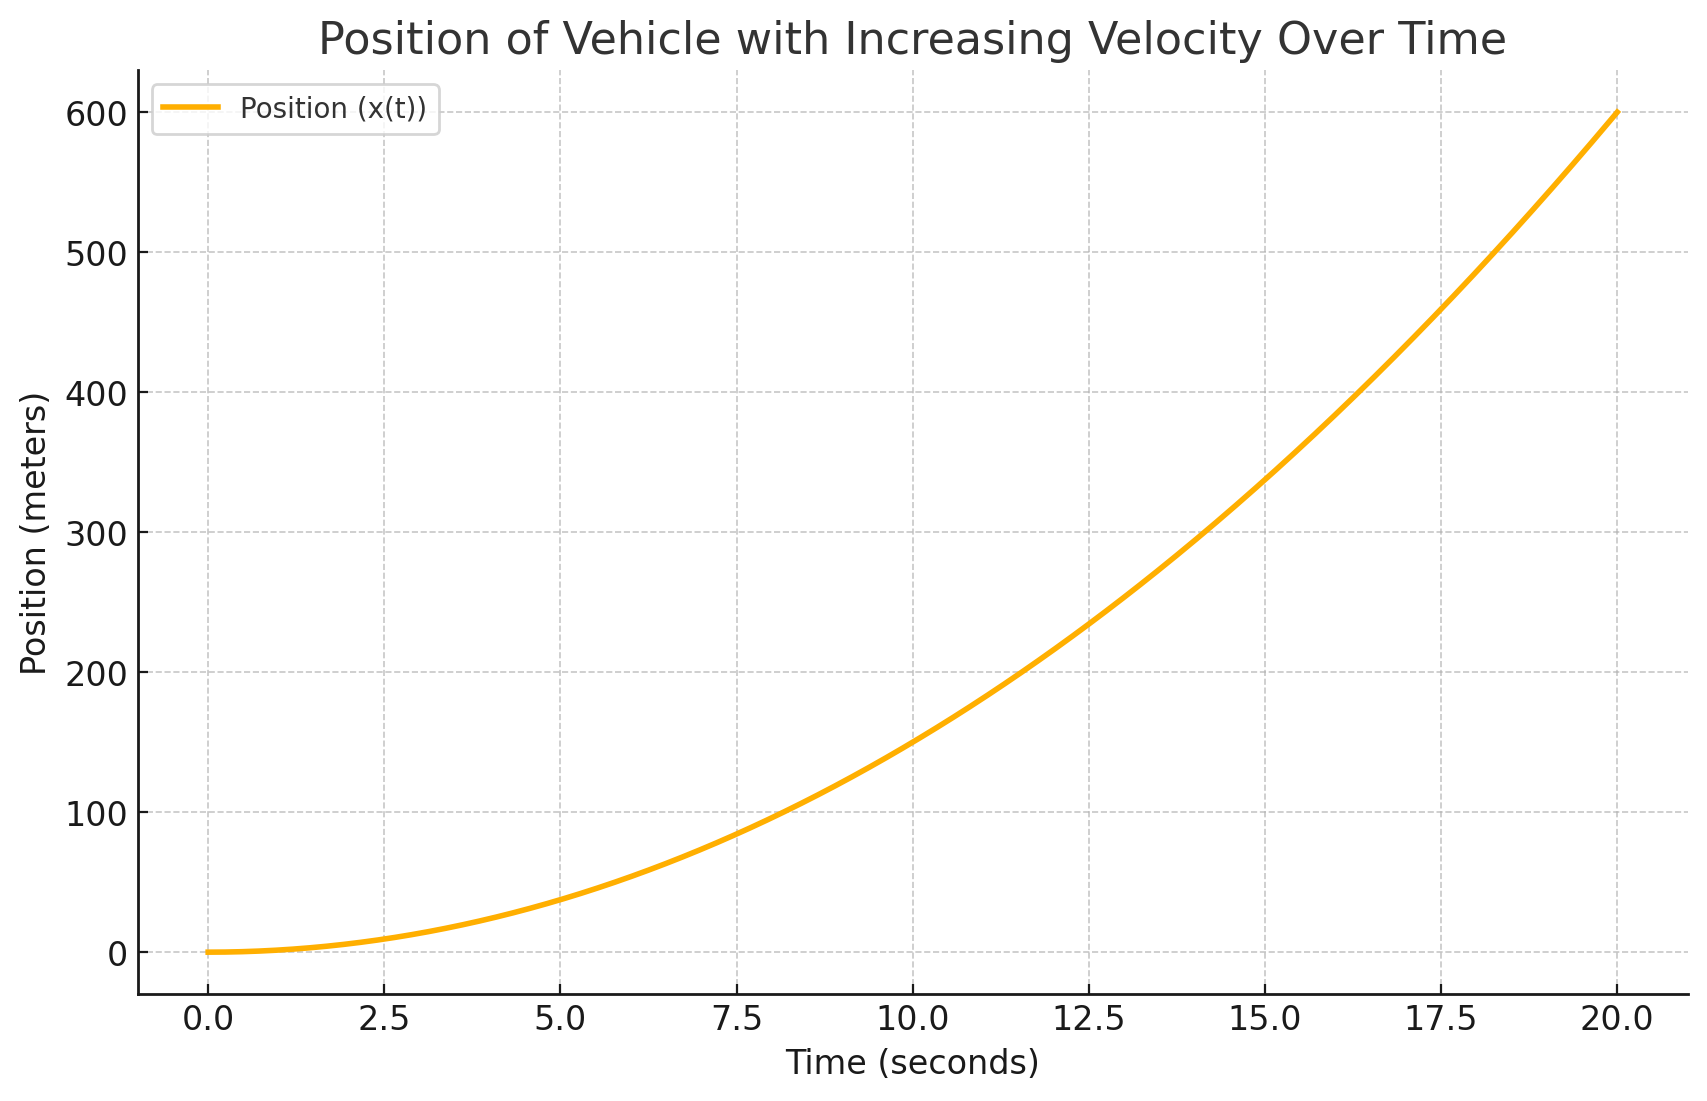
\includegraphics[width=\textwidth]{graphs/position.png}
  \caption{Position over time graph}
  \label{fig:position_graph}
\end{figure}

\begin{figure}[H]
  \centering
  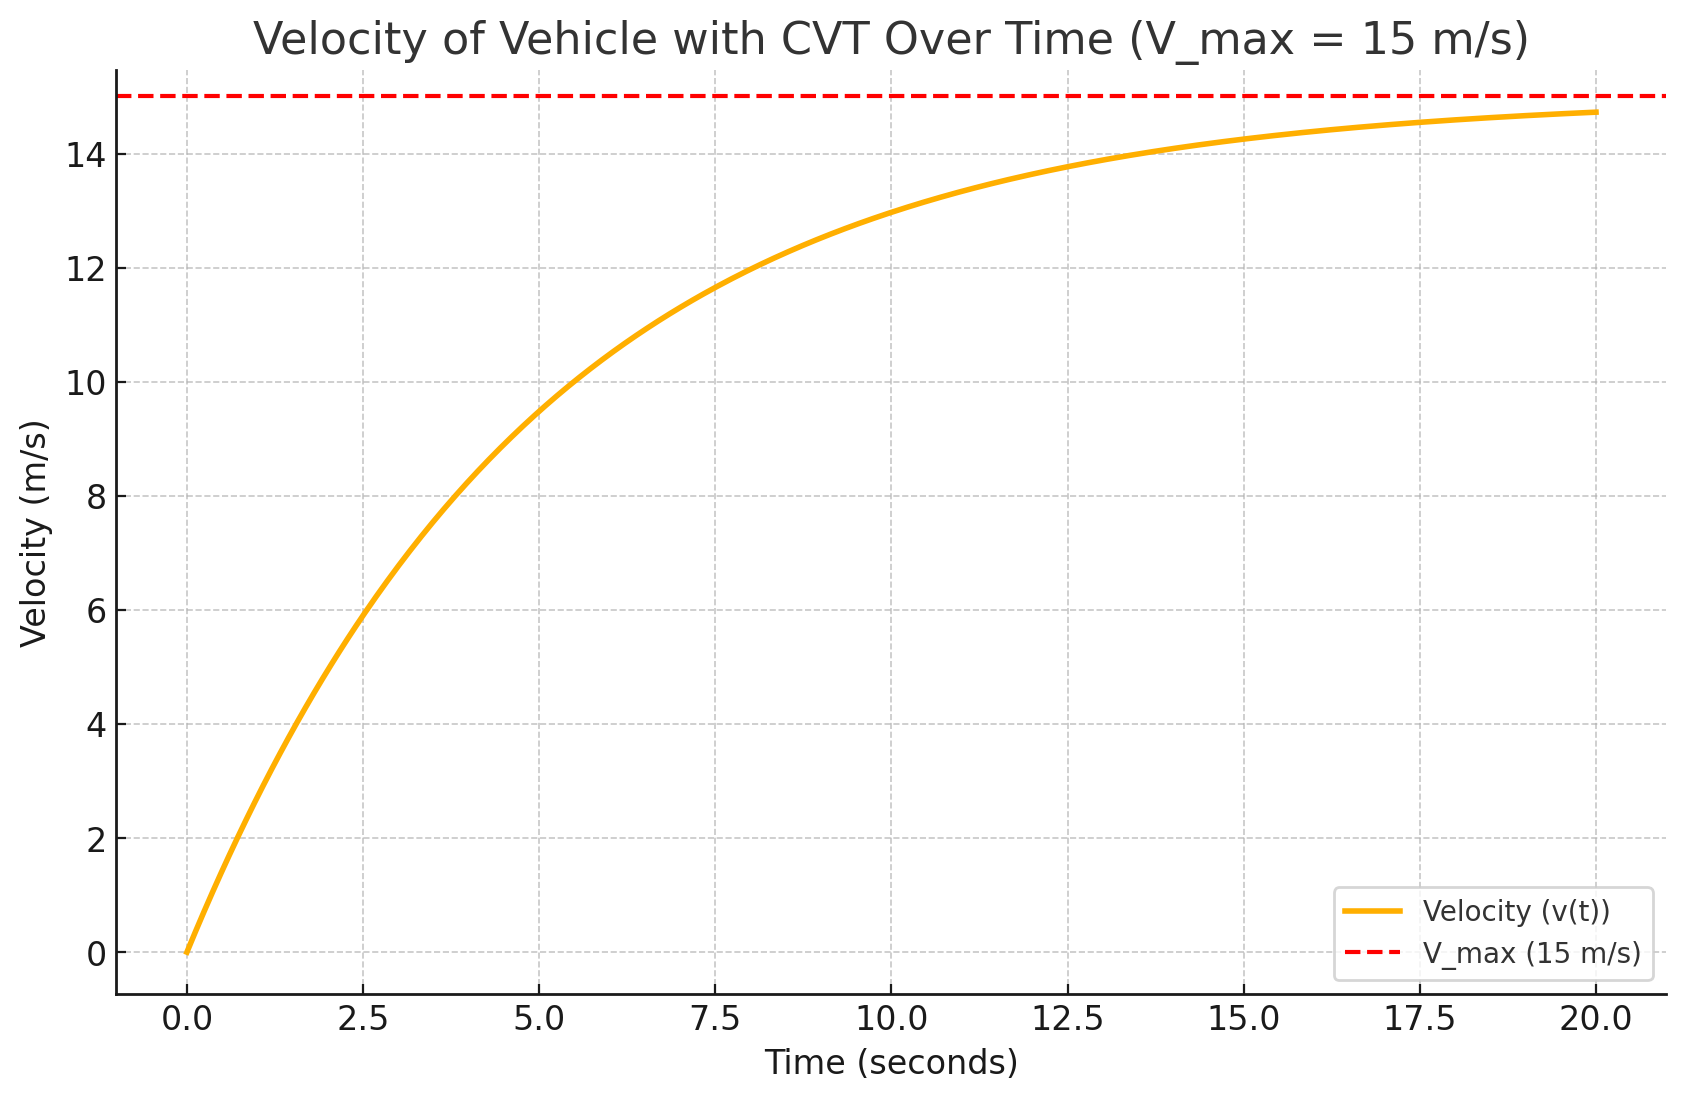
\includegraphics[width=\textwidth]{graphs/velocity.png}
  \caption{Velocity over time graph}
  \label{fig:velocity_graph}
\end{figure}

\begin{figure}[H]
  \centering
  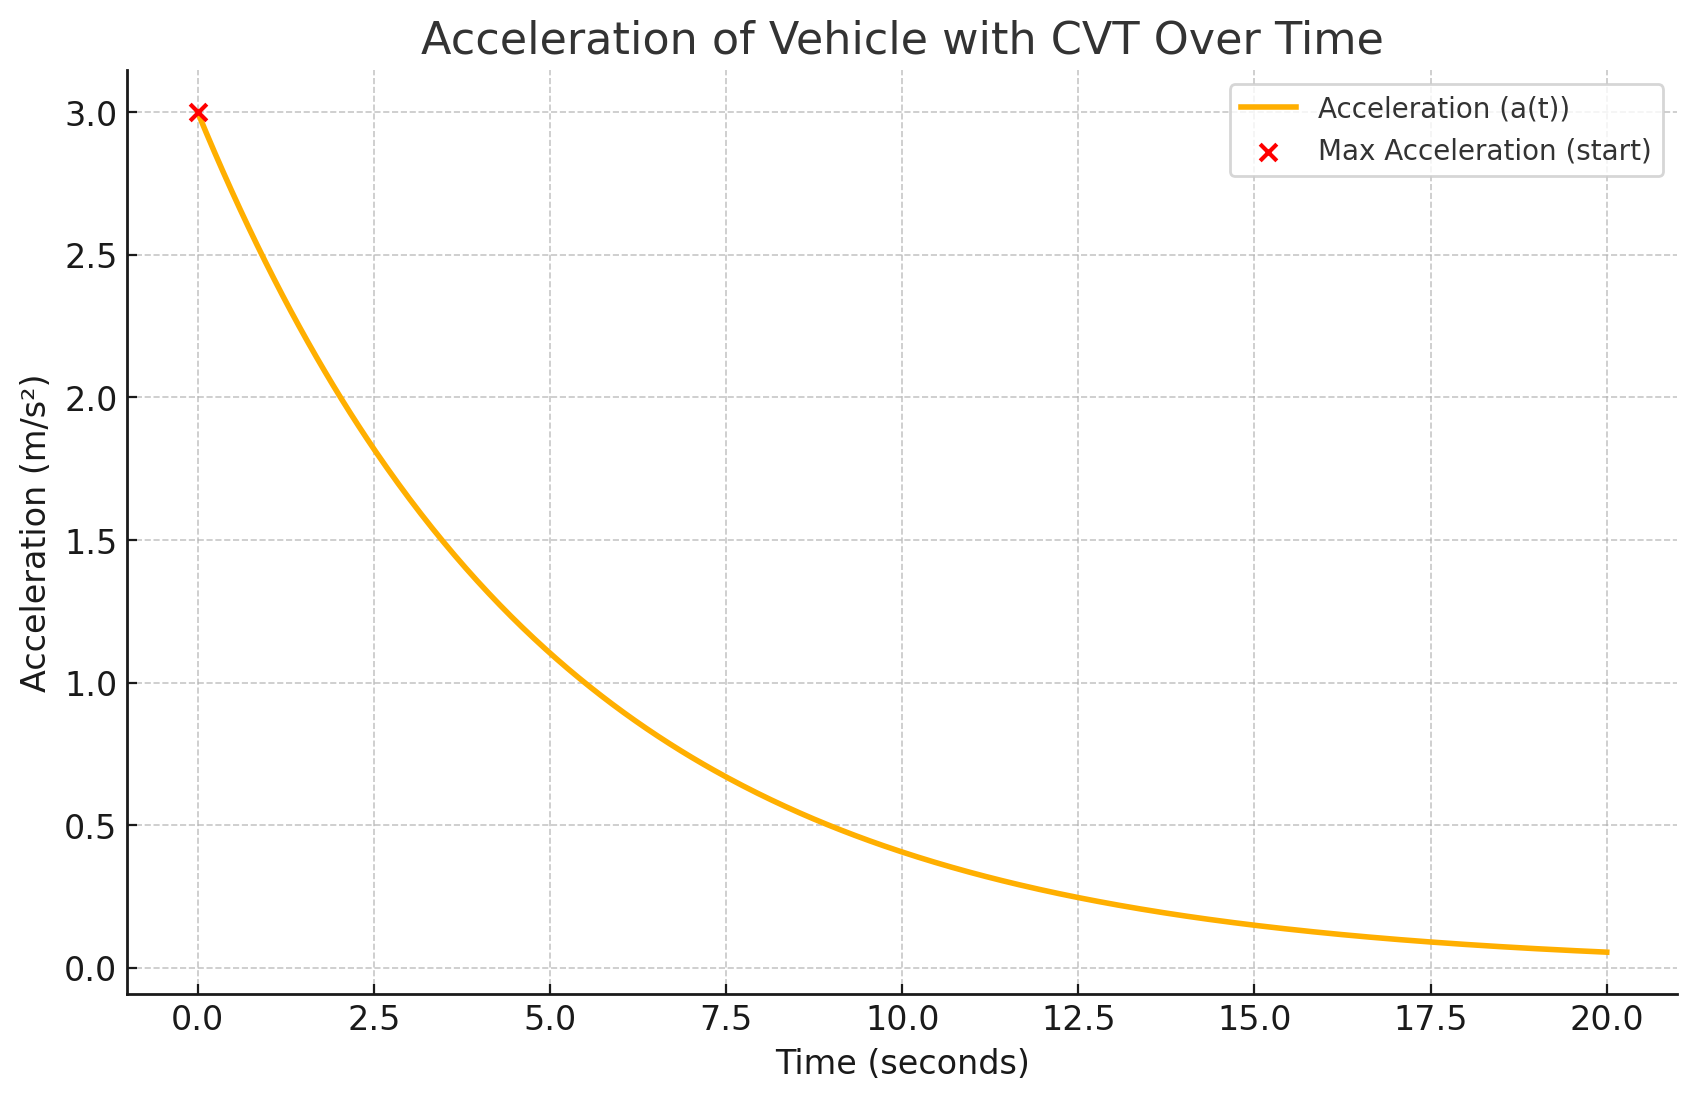
\includegraphics[width=\textwidth]{graphs/acceleration.png}
  \caption{Acceleration over time graph}
  \label{fig:acceleration_graph}
\end{figure}

\begin{figure}[H]
  \centering
  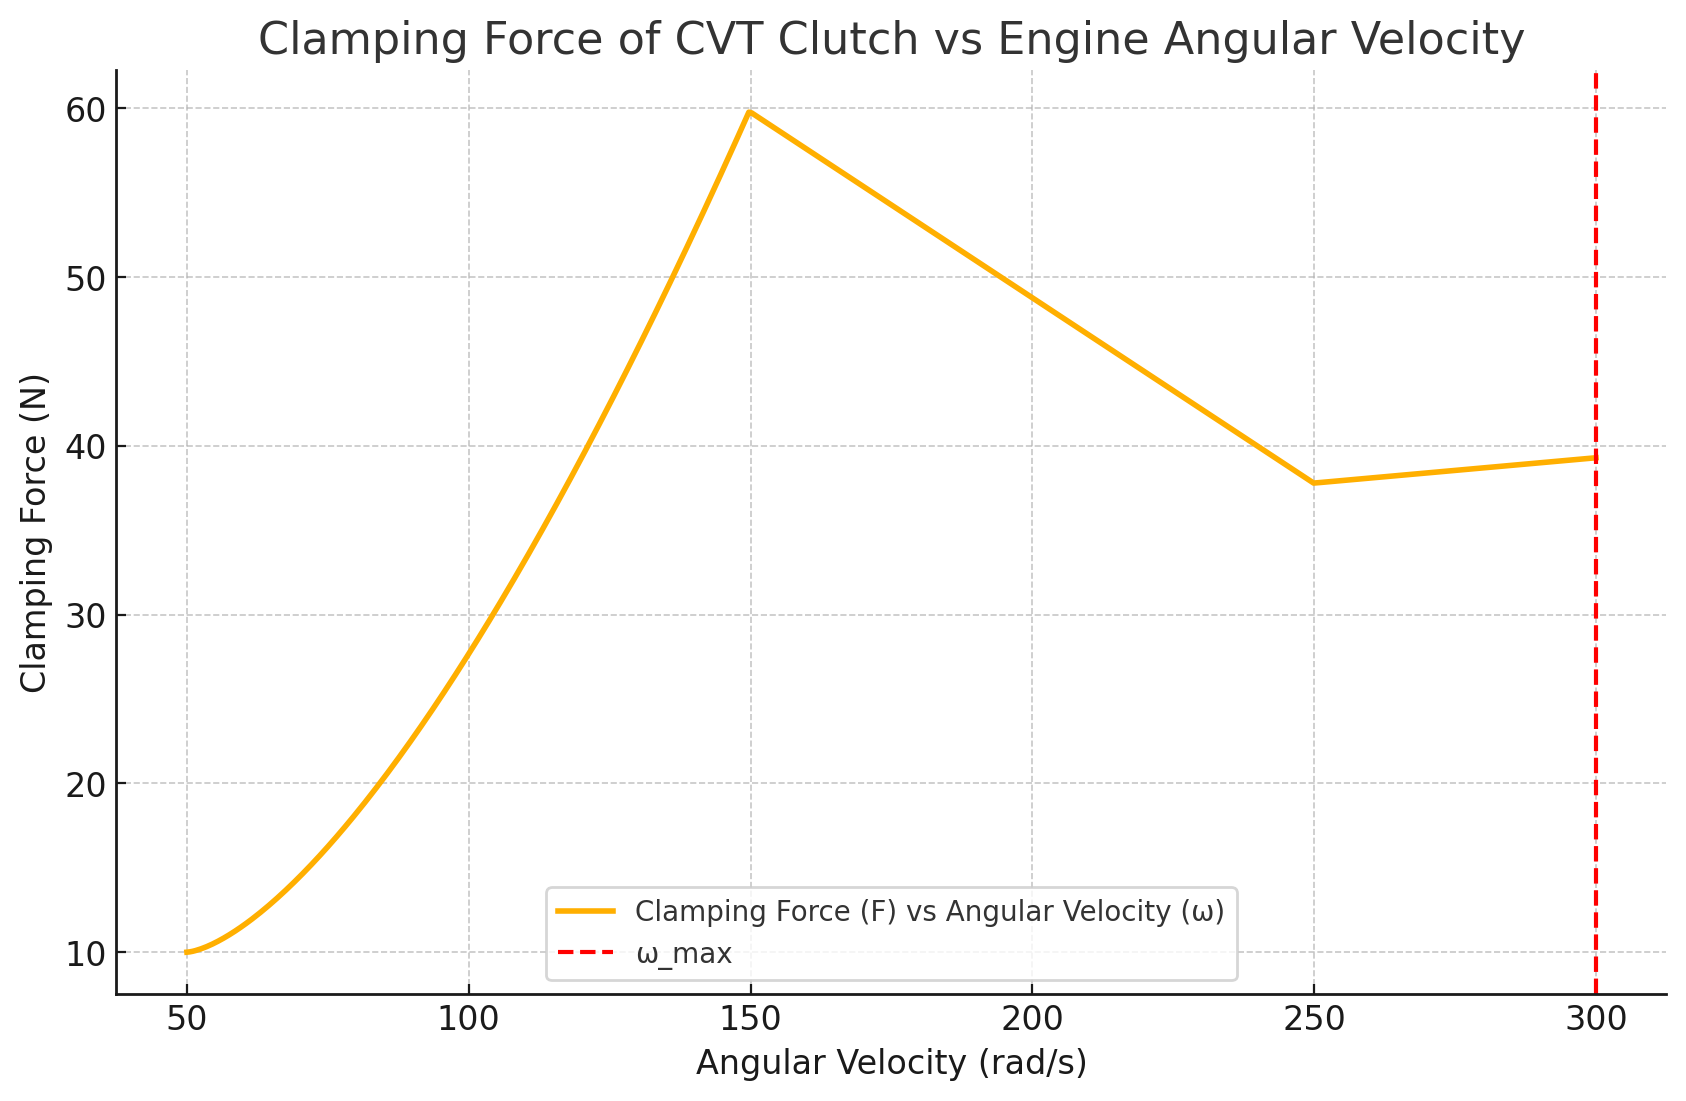
\includegraphics[width=\textwidth]{graphs/clamp_force.png}
  \caption{Clamping force against engine angular velocity graph}
  \label{fig:clamping_force_graph}
\end{figure}

\begin{figure}[H]
  \centering
  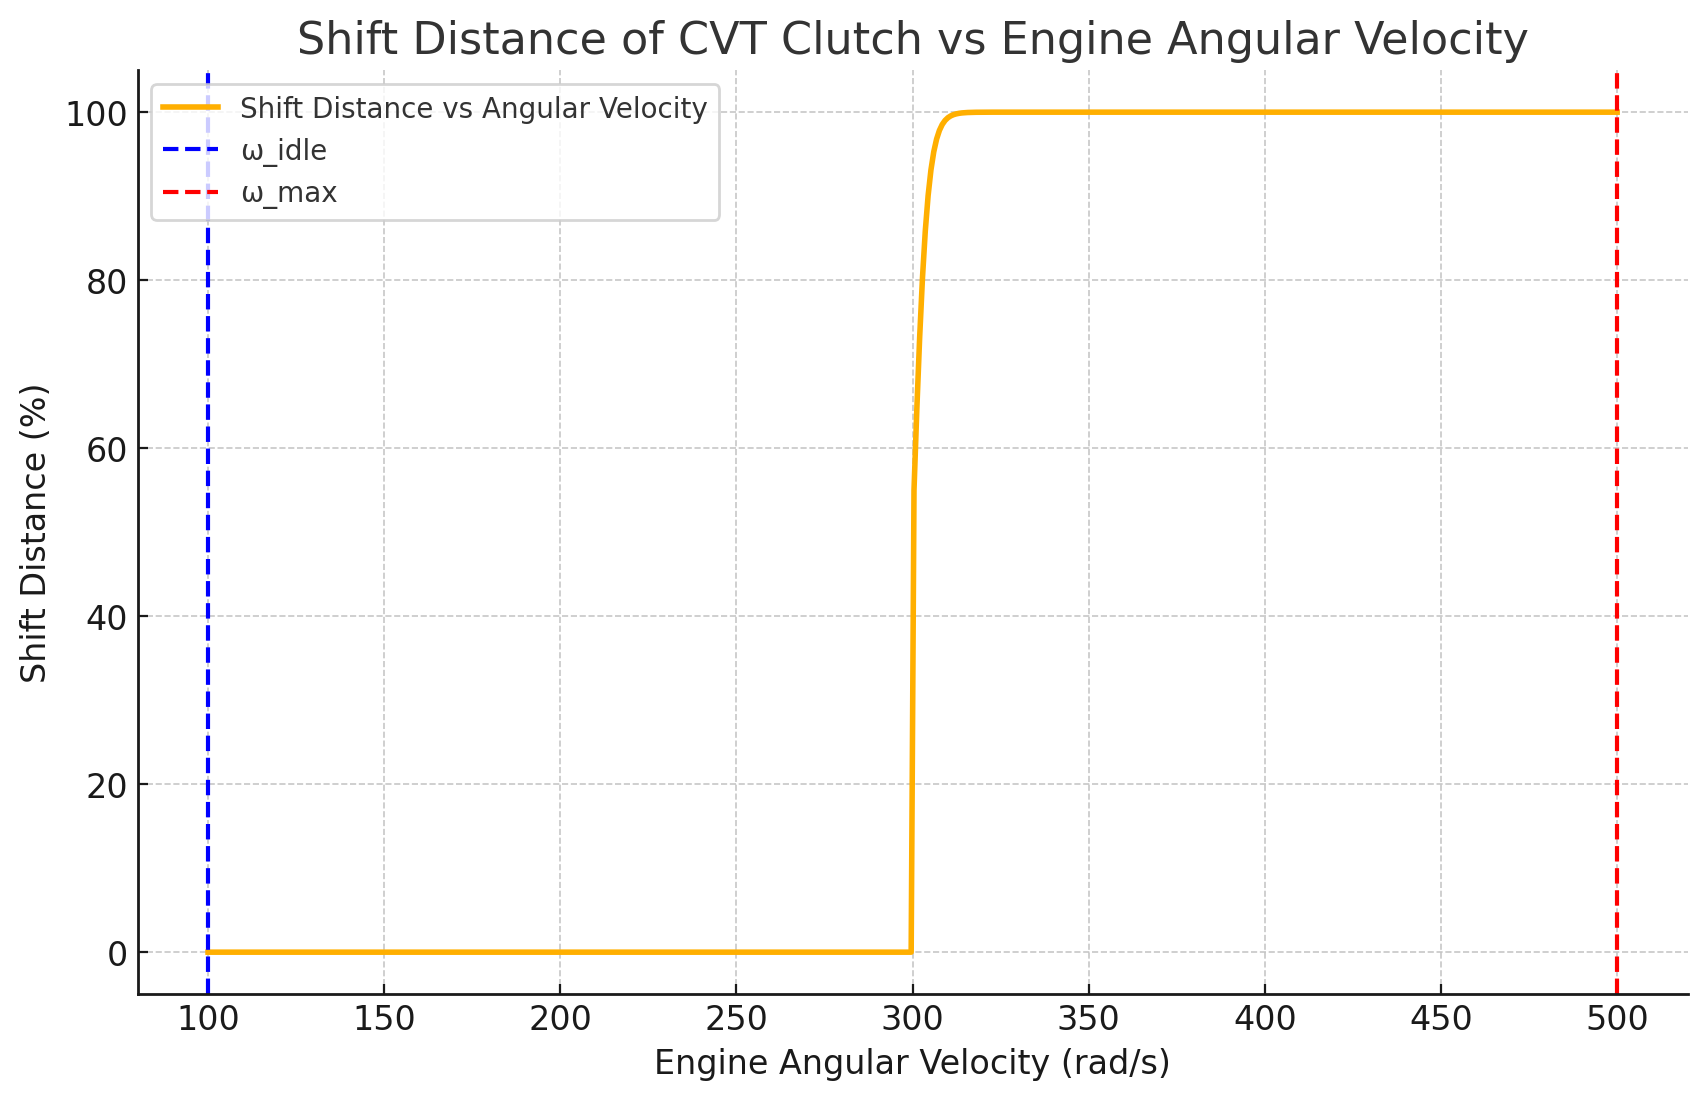
\includegraphics[width=\textwidth]{graphs/shift_vs_engine.png}
  \caption{Shift distance against engine angular velocity graph}
  \label{fig:shift_distance_graph}
\end{figure}

\begin{figure}[H]
  \centering
  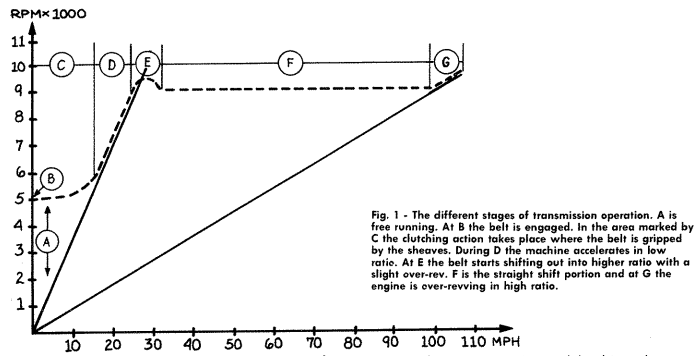
\includegraphics[width=\textwidth]{graphs/shift_curve.png}
  \caption{Shift curve graph \citet{Aaen2007}}
  \label{fig:shift_curve}
\end{figure}

\subsubsection*{B / C - Clutching}

Belt engagement starts with a lot of slip when the vehicle is stationary, increasing to 100\% engagement when the vehicle is accelerating along the low ratio line. In between these two points there is slippage between the belt and the sheave. After the flyweight force overcomes the spring tension, the RPM has to increase and give more sheave pressure on the belt until there is no slippage and full engagement. This takes place as the vehicle is starting to move and as the engine speed and vehicle speed intersect at the low ratio line. This area is often critical for good and smooth take-off. Incorrect matching of springs and weights may lead to excessive slippage and belt wear.

\textbf{The clutching phase begins when the flyweight force overcomes the pretension, and lasts until the flyweights have generated enough side force to transfer the engine torque without slipping the belt.}

\subsubsection*{D - Low Ratio Acceleration}

After the sheaves have gripped the belt and they are transferring the torque without slipping, the machine will accelerate along the low ratio line. The engine speed will continue to increase as if you were in low gear in your car. While the vehicle speed is increasing the belt remains in low ratio at the bottom of the driving sheaves. The belt will not start moving out on the sheave until the flyweight force has become large enough to overcome both the pressure spring and the side pressure of the belt on the driven sheave. When the engine speed has built up to create enough centrifugal force to overcome the pressure spring and the driven sheave pressures, the belt will start shifting out and the ratio will change. This is called the “shift point” and should coincide with the power peak of the engine.

\textbf{Between full engagement and the shift point, centrifugal forces are larger than the pressure spring but less than the belt pressure from the driven clutch.}

\subsubsection*{E - Shift-Out-Point}
As the RPM of the driving clutch increases in low ratio, the centrifugal force from the flyweights will eventually be large enough to overcome the tension on the belt from the driven clutch. When this occurs, the transmission has reached the shift out point and the belt will start to move outward on the driving clutch and inward on the driven clutch. As the belt starts to move, the drive ratio is changed.

Ideally, the shift out point should be at the power peak of the engine and the shift curve should be straight from there through high ratio. In practice it may sometimes end up a little different. If you have a heavy machine and a small high revving engine, you may want the shift out point to be several hundred RPMs higher than the power peak. As the machine increases acceleration the engine may be pulled down in RPM by the increasing load as the transmission shifts out. By over-revving slightly in the beginning the engine will be pulled down on to the power peak, and smooth acceleration continues. If the shift out point was right on the power peak, the reduction in RPM would have pulled the transmission down off the peak and a more sluggish acceleration would have occurred as the transmission worked its RPM up again.

This shift out over-rev is of short duration, and highly individual depending on the combination of machine weight and engine power. On a super light drag machine with a big engine, you may get away with starting the shift-out slightly before the power peak as the power will pull you right through without an RPM drop. The best way to achieve the initial over-rev is to modify the shift curve of the flyweight right off the engagement point. This is usually done by extending the engagement flat into the shift curvature. The length and shape of the transition from engagement to shift curve will determine the amount and duration of the shift out over-rev.

\textbf{The shift out point occurs when the flyweight force overcomes the belt pressure from the driven clutch.}

\subsubsection*{F - Straight Shift}

The ideal shift-curve is “straight” between the low and high ratio. This means that the engine speed is held constant at the power peak while the transmission is shifting out and the vehicle speed is increasing. With the exception of a slight shift-out over-rev as discussed in the previous section, a straight shift at the power peak will give the maximum performance. To maintain a straight shift is not an easy task. As we saw under the discussion of the belt pressure requirements, the pressure on the belt is actually decreasing as the transmission shifts out. This decrease in belt tension may be as much as 50% between low and high ratio. If the decrease is not matched by the flyweight force, the driving clutch will compensate by lowering the engine speed. The driving clutch will always match the required belt tension by changing the engine speed if the flyweight system is not correctly calibrated. Our task is to make sure the flyweight system matches the belt forces at the peak power engine speed. Straight shifting is accomplished by calibrating the relationship of the flyweight curvature and roller location as well as the arc traveled by the flyweight. Engine speed is determined by the weight of the flyweight system.

Since the flyweight system works against the pressure spring in the driving clutch, the loads and rates of this spring also influence straight shift and engine RPM. Flyweight curvatures have been experimented with and fine tuned by the manufacturers over the last 15 years and they provide a good selection of tuning components. Polaris is a good example; they provide two basic flyweight curvatures, trail and racing. The trail curvature has lower engagement and softer shift-out than the racing curvature. Each flyweight group is available with weights in 2-4 gram increments for each curvature. Each manufacturer also has a large selection of springs with different pretensions and rates for calibration purposes. Achieving the correct combination of flyweight and spring to obtain a straight shift at the correct engine speed is the task of the tuner. This will be covered in greater detail under the Selection of Components and Testing chapters.

\textbf{Straight shift is obtained by matching curvature and spring rates; correct engine speed is dependent on the weight of the flyweight.}

\subsubsection*{G - Over-Run}

When the transmission is shifted all the way out into high ratio, engine speed must increase along the high ratio line as vehicle speed increases.

As the engine speed increases, the power curve goes off the peak on the back side and less power is available to propel the machine. Maximum speed cannot be obtained if you are off the peak; this means the machine is geared too low. There may be conditions where this is done on purpose because acceleration is more important than top speed. In most cases the machines are geared to give maximum top speed, which means they will seldom reach high ratio and over-run is not usually experienced.

\textbf{In over-run, the clutches are shifted all the way out and the flyweight forces have no more influence on the engine speed. Engine speed will increase along the fixed high ratio line.} \citet{Aaen2007}

\begin{figure}[H]
  \centering
  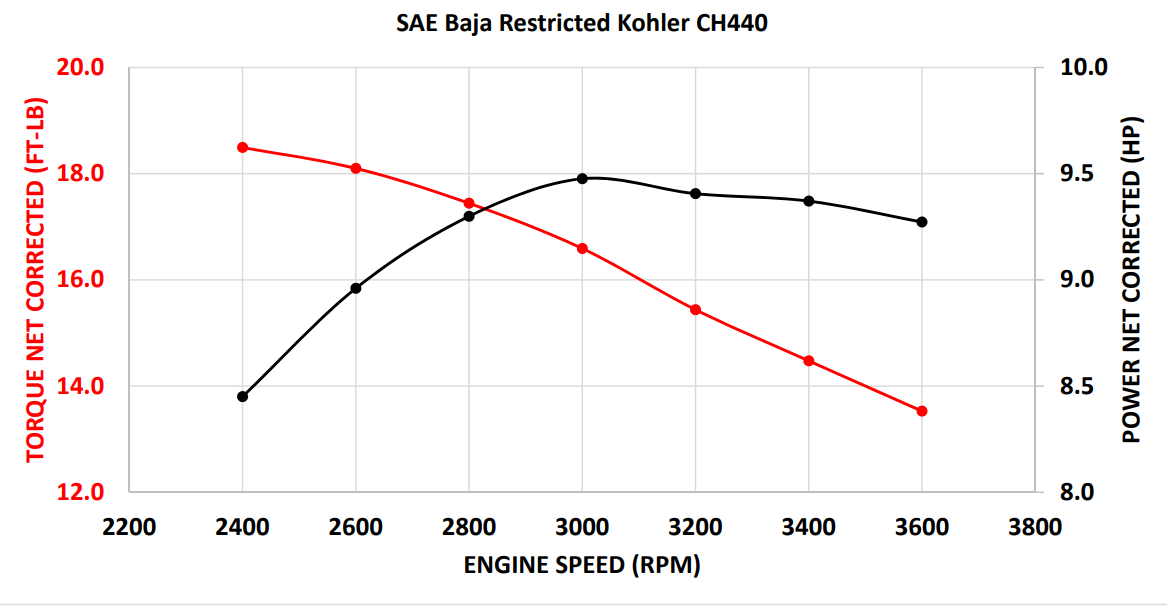
\includegraphics[width=\textwidth]{graphs/engine.png}
  \caption{Engine torque and power against engine angular velocity \citet{BajaSAEKohlerEngine2022}}
  \label{fig:engine_graph}
\end{figure}

\newpage{}
\section*{Appendix --- Reflection}

The information in this section will be used to evaluate the team members on the
graduate attribute of Lifelong Learning.

\input{../Reflection.tex}

\begin{enumerate}
  \item What went well while writing this deliverable?\\ 
  When writing this deliverable there was a lot of things that went well.
  Firstly the team had a long sitdown with our capstone supervisor Dr Smith to discuss the process of how we will be validating our simulation.
  We were able to come up with a great plan for how the simulation will be validated against real world data and how to incorperate that into this document and the project as a whole.
  The team was also able to have some great communication with each other when figuring out how to write the various kinds of tests for the system.
  Since there was a lot of different types of tests we were constantly bouncing ideas off each other to figure out the best way to move forward.
  Team communication such as that is always a good thing and this deliverable specifically had a lot of that in it.
  Another thing that went well was the team was able to figure out who on the McMaster Baja team will help us validate our simulation once the implementation is complete.
  We outlined a list of people that will help us in section 3 of this document and we were able to get in contact with them and they are all on board to help us validate the simulation.  

  \item What pain points did you experience during this deliverable, and how
    did you resolve them?\\
    When writing this deliverable there was only one pain point that needed to be resolved.
    The first one was how to write the functional tests for the math component of the system.
    Due to the nature of our project the simulation outputs are not something that will be able to be verified/validated numerically or with a simple test.
    Instead we will need to compare the outputs of the simulation to the outputs of the physical car.
    Therefore we had to change the way that we wrote the functional requirements, and instead of writing them as a simple test we wrote them as a comparison between some specific part of the simulation output and against the same data gathered from the physical car.
    The way this pain point was resolved was through sitting down with our capstone supervisor Dr Smith and talked the process of how we will be validating our simulation and he was the one who gave us the reccomendation to write the functional requirements in this way.
  \item What knowledge and skills will the team collectively need to acquire to
  successfully complete the verification and validation of your project?
  Examples of possible knowledge and skills include dynamic testing knowledge,
  static testing knowledge, specific tool usage, Valgrind etc.  You should look to
  identify at least one item for each team member.

  In order to successfully complete the verification and validation of our project the team will need to acquire various knowledge and skills regarding testing.
  Some areas that we will need to gather skills in will be in areas of testing such as dynamic testing, static testing, unit testing and system testing. 
  As well the team will need to learn how to use specific tools for the various languages that we will be using.
  For python this will include:
  \begin{itemize}
    \item coverage
    \item unittest
    \item Flake8 (linter)
    \item black (code formatter)
  \end{itemize}
  For C\# this will include:
  \begin{itemize}
    \item SonarLint
    \item StyleCop
    \item UTF (Unit Test Framework)
    \item UTR (Test framework for Unity)
  \end{itemize}

  As well beyond testing tools and knowledge the team will also have to get familiar with how to validate the simulation output against the physical car data. 
  This involves working with the McMaster Baja teams data acquisition system to gather the data from the car and then how to compare that data to the simulation output.
  This will involve understanding different types of data involved with the CVT that were outlined in section 4 and learning what a correct graph of those kinds of data look like.
  
  Team skill breakdown
  \begin{itemize}
    \item Travis: Need to familiarize himself with the C\# testing tools and how to use them. As well he will need to learn how to validate the simulation output against the physical car data.
    \item Grace: Need to familiarize herself with the C\# testing tools and how to use them. As well she will need to learn how to validate the simulation output against the physical car data.
    \item Kai: Need to familiarize himself with the Python testing tools and how to use them. He is already familiar with the data acquisition system and how to gather data from the car.
    \item Cam: Need to familiarize himself with the Python testing tools and how to use them. He is already familiar with the data acquisition system and how to gather data from the car.
  \end{itemize}
  \item For each of the knowledge areas and skills identified in the previous
  question, what are at least two approaches to acquiring the knowledge or
  mastering the skill?  Of the identified approaches, which will each team
  member pursue, and why did they make this choice?

  One way to acquire the knowledge and skills needed to successfully complete the verification and validation of our project is to take watch some videos online about how to use them.
  There are many videos that are available that can teach you how to use the various testing tools that we will need to use.
  Another way to acquire the knowledge is to read the documentation for the tools libraries that we are going to use.
  This would involve reading the documentation for the testing tools that we will be using and learning how to use them from there.
  After reading some documentation you can then try to implement the tools in a small project to get a feel for how they work.

  Each team member will be using the second approach to acquire these knowledge and skills. 
  We felt that the best way to learn testing tools is to read the documentation on how they should be used.
  Then once we are implementing the POC we can use that smaller project to get a feel for how the tools work and how to use them.
  This will gives us the base knowledge and the practicality of how to use the tools in a real project.
\end{enumerate}

\end{document}